\clearpage

\section{CAPEX}
\begin{tcolorbox}	
\begin{tabular}{p{2.75cm} p{0.2cm} p{10.5cm}} 	
\textbf{Student Name}  &:& Tiago Esteves    (October 03, 2017 - )\\
\textbf{Goal}          &:& Implement of the heuristic model to obtain the best possible CAPEX of a given network.
\end{tabular}
\end{tcolorbox}
\vspace{11pt}

The total CAPEX of a network, as it was already described in \ref{Capex}, is the sum between two differentiated costs. Firstly, the link cost depends on the link length, which has integrated components such as the OLT, transponders and amplifiers and the node cost depends on the traffic intensity by each node. The optical node cost is 0 because all the ports in the network are electrical.

In order to get the results for the heuristic approach, several algorithms are used which try to obtain the most near optimal solution for the six cases detailed in this chapter. The first step is to create the ODU matrices in the Net2Plan network design software as it is described below.

\subsection{Creation of traffic matrices}\label{creation_traffic_matrices}

Accordingly to the reference network in \label{Reference_Network_Traffic} and to the ODUs defined in \label{low_traffic_scenario} for the low, medium and high traffic scenario, we can create the traffic matrices with a constant traffic pattern. As all the network components are bidirectional, the amount of traffic that passes to all node pairs must be the same.

The next step is to choose the number of nodes, number of matrices and the constant value. For the network of reference it is used 6 nodes, 5 matrices and the constant has value 0. After inserted the values in each ODU matrix it is possible to save them and create now a network topological design.

\begin{figure}[h!]
\centering
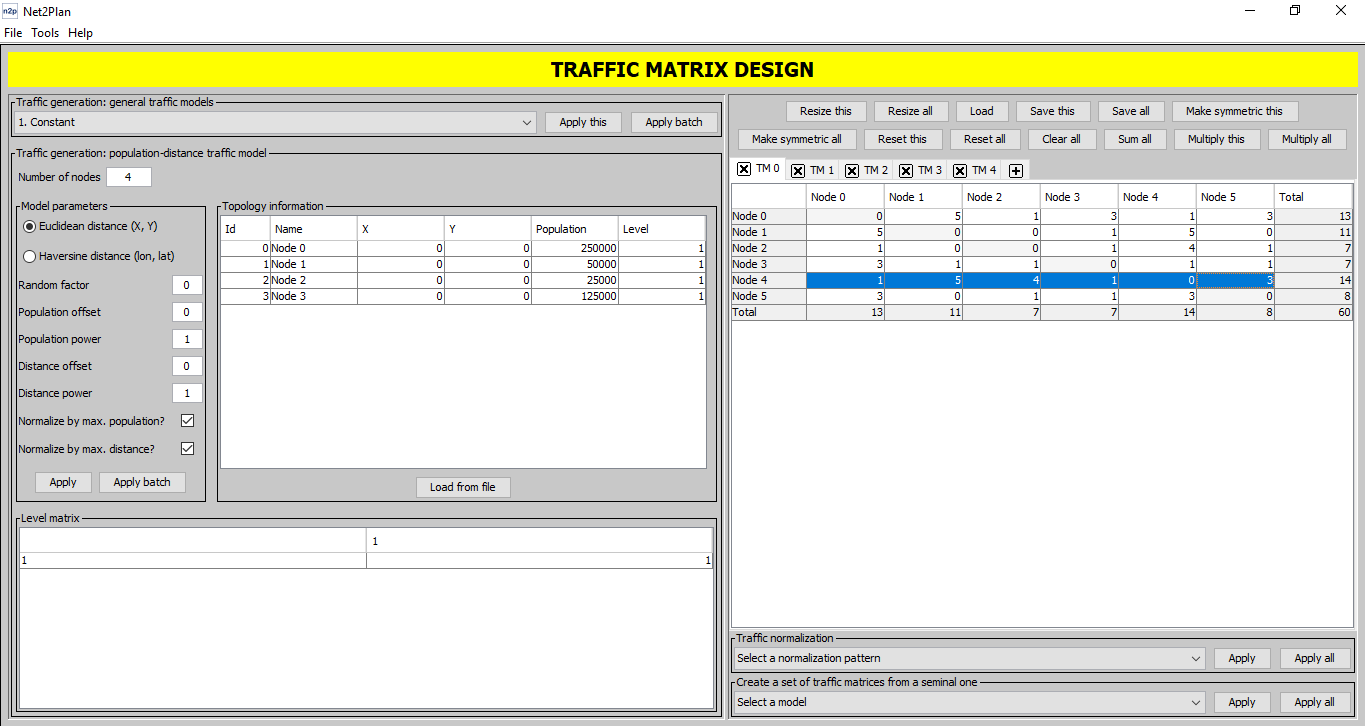
\includegraphics[width=12cm]{sdf/heuristic/figures/traffic_matrix_design}
\caption{Traffic matrix design using Net2Plan.}
\label{traffic_matrix_design}
\end{figure}

\subsection{Creation of a network topological design}\label{creation_topological_design}

\vspace{11pt}
To create the network topological design that was defined before in \label{creation_traffic_matrices} it is needed to add the 6 nodes that were chosen and link them with bidirectional links as it is shown in the picture \label{network_topological_design} below.

On the right side of the network design it is shown all the attributes of the network. However, some arguments are not set yet, like the capacity and the traffic demands that passes in each link, so now it is necessary to use routing and grooming algorithms in order to simulate the heuristic algorithms in this reference network.

\begin{figure}[h!]
\centering
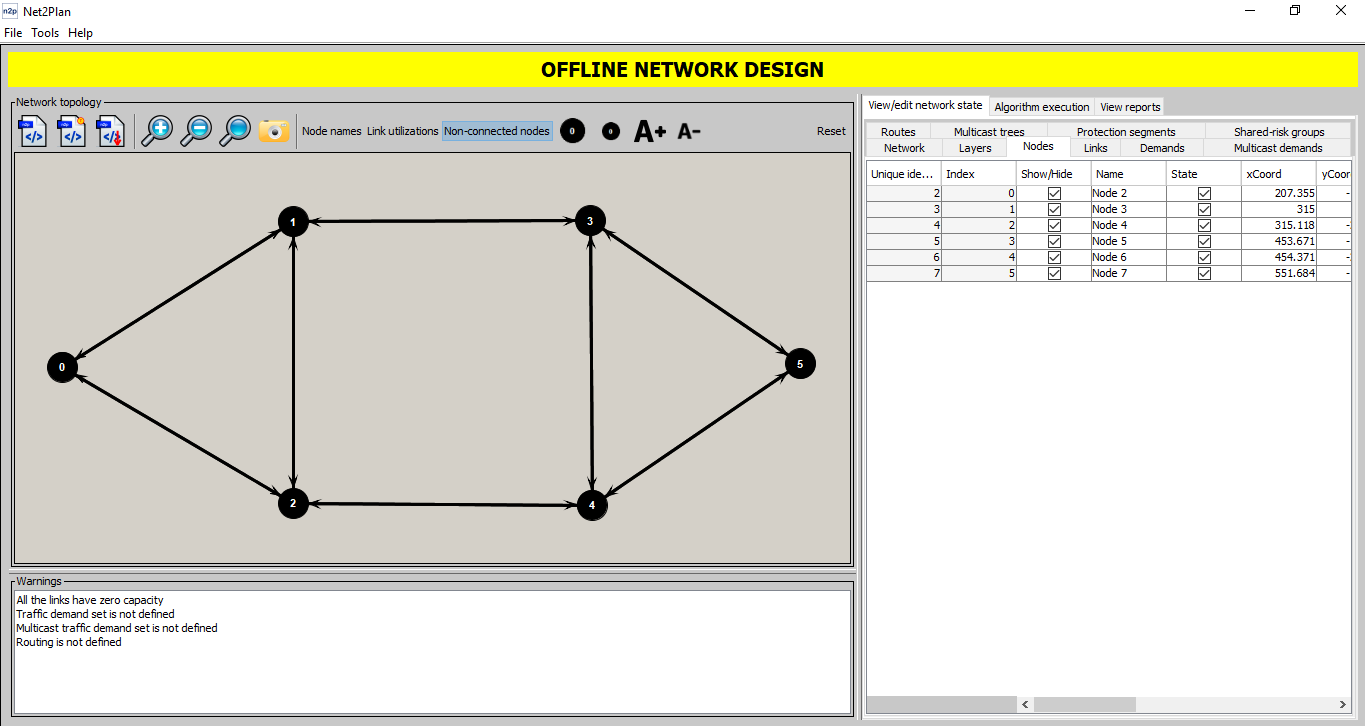
\includegraphics[width=12cm]{sdf/heuristic/figures/network_topological_design}
\caption{Network topological design using Net2Plan.}
\label{network_topological_design}
\end{figure}

\subsubsection{Join Traffic Matrices Algorithm}\label{join_traffic_matrices_algorithm}

\vspace{11pt}
The first algorithm used is the "Join Traffic Matrices" algorithm and it joins the traffic demands of the ODU traffic matrices into a file. This file will be used later for loading the traffic demands to the network topological design on Net2Plan. This algorithm aggregates the traffic matrices from ODU0 to ODU4. If it is used a network with multiple matrices and, respectively, multiple traffic demands it is possible to join each of them and save it.

\clearpage
\begin{figure}[h!]
\centering
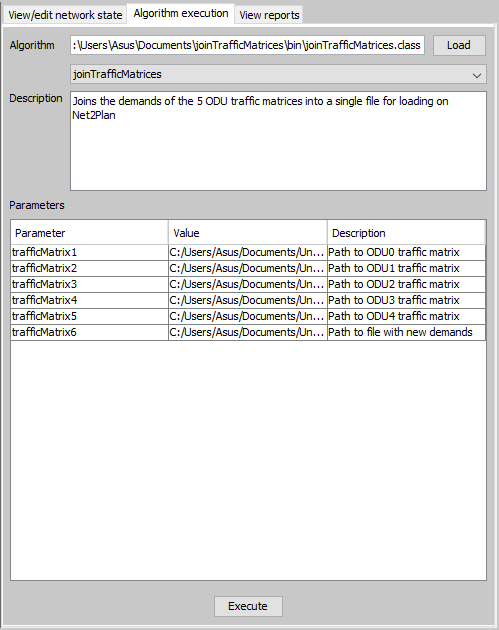
\includegraphics[width=10cm]{sdf/heuristic/figures/join_traffic_matrices}
\caption{Join traffic matrices algorithm using Net2Plan.}
\label{join_traffic_matrices}
\end{figure}

\subsubsection{Logical Topology Algorithm}\label{logical_topology_algorithm}

\vspace{11pt}
The "Logical Topology" algorithm is the second one used and it is based on the transport mode that is used in the network and it creates the logical topology on another layer. The logical topology value is introduced by the user and it can be one of the three transport modes available. If the transport mode chosen is opaque there is no need of having a second layer because the logical layer is the same as the physical one and if the transport mode is transparent or translucent it is needed to add a new logical layer. One advantage of this algorithm is that all the traffic demands are copied to the new layer and all the arguments remains the same depending on the previous layer, not interfering with the network topology.

It is also needed to add by the user the capacity that is used in each wavelength from all origin nodes to all destination nodes and the length of the links with values of the distance matrix represented in \label{Reference_Network_Topology} and expressed in Km.

\begin{figure}[h!]
\centering
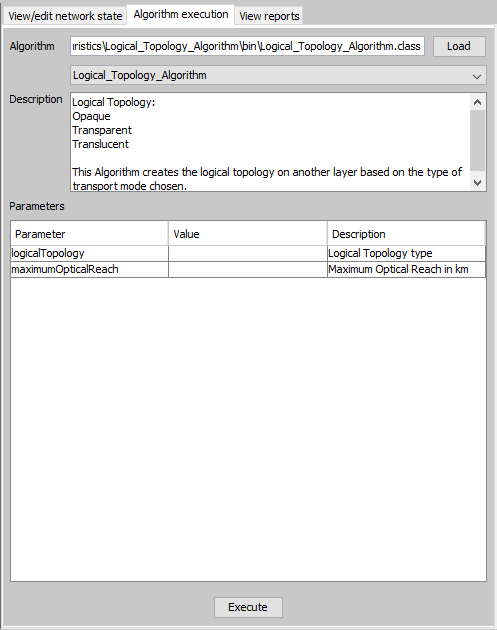
\includegraphics[width=10cm]{sdf/heuristic/figures/logical_topology}
\caption{Logical topology algorithm using Net2Plan.}
\label{logical_topology}
\end{figure}

\subsection{Grooming Algorithm}\label{grooming_algorithm}

\vspace{11pt}
The "Grooming" algorithm is a shortest-path heuristic algorithm that creates routes and protection paths based on hops or km, accordingly to the pre-defined logical topology. The goal of this grooming algorithm is to minimize the number of links for each path between all node pairs and this will lead to the reduction of the number of wavelengths to serve a set of connections and, consequently, to a lower cost of nodes and lower CAPEX.

The approach of the routing algorithm is to route all the traffic demands using the "Dijkstra" algorithm and uses the shortest number of hops to reach the destination node. The shortest path between two nodes is the one that includes connections whose sum of weights is the least possible. Routing through the shortest path consists in routing sequentially each element of a traffic matrix to the shortest path in the network. The routing is done in the logical and physical topologies of the network. In addition, the route from node o to d should be the opposite direction of node d to o as there could be different routes with the shortest path that are not using the same path. It is assumed that links are bidirectional and the traffic demands are given between pairs of nodes and a network topology. In this case, each wavelength will be served by two wavelength paths. If the number of used wavelengths is minimum, the number of used fibers will be also minimum, which minimizes the CAPEX.

The 1+1 protection scheme (dedicated path protection) assumes that each link has a dedicated protection communication channel. For this scenario, it is necessary to assign different wavelengths to the primary and protection paths. It is chosen the best path based on the shortest or disjointed path, for without survivability or with 1+1 protection, respectively. The optimization objective is to minimize the number of assigned wavelengths and network components.

\begin{figure}[h!]
\centering
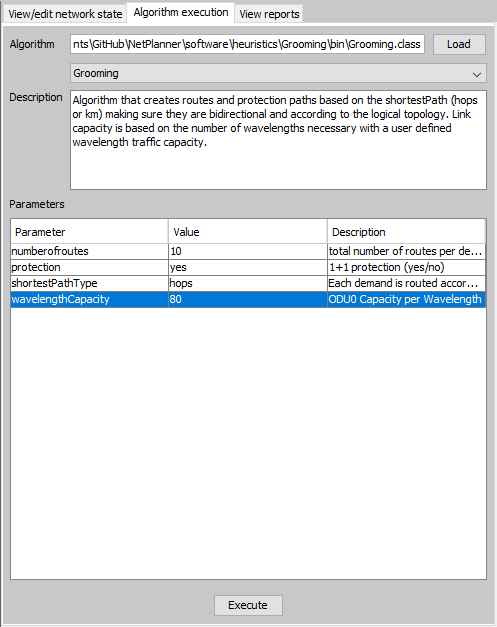
\includegraphics[width=10cm]{sdf/heuristic/figures/grooming}
\caption{Grooming algorithm using Net2Plan.}
\label{grooming}
\end{figure}